% this is source code for one of the sessions in Digital Skills for Research Workshop (EMTTI, University of Wolverhampton)
% March 2022, Maria Kunilovskaya (mkunilovskaya@gmail.com)

\documentclass[a4paper,11pt]{article}
\usepackage[utf8]{inputenc}  % file encoding

\usepackage[T1,T2A]{fontenc}  % char encoding for Latin and Cyrrilic
\usepackage[spanish,english]{babel} % support for another language; all automatic captions are generated in Eng as the main lang for this doc

% custom colours for various types of links
\usepackage[colorlinks=true, linkcolor=blue, urlcolor=cyan, filecolor=magenta]{hyperref} 

% margins and layout
\usepackage{geometry}
\geometry{
	a4paper,
	total={170mm,257mm},
	left=20mm,
	top=15mm,
}
\setlength\parindent{0pt} % set all indents to 0
% print several lines of code verbatim
\usepackage{listings}

% draw a colored box
\usepackage{tcolorbox}

% this redifines \href which by default adds .pdf if it does not see a recorgnisable file extension, wich is the case when a folder is passed
\makeatletter
\newcommand\HREF[2]{\hyper@linkurl{#2}{#1}}
\makeatother

% heading of a document
\title{Session 7. Reference management: Mendeley}
\author{Digital Skills for Research}
\date{March 23, 2022}

\begin{document}

\maketitle
\tableofcontents

\section*{Some points covered in previous Week 3}
\addcontentsline{toc}{section}{Some points covered in previous Week 3}

Reflect on your progress and see whether you can recall these learnables:

\bigskip

\tcbset{colback=blue!5!white,colframe=blue!50!black!40}
\begin{tcolorbox}[width=.475\textwidth, nobeforeafter,height=6.5cm,valign=center, fonttitle=\bfseries,title=Session 5]
	\begin{enumerate}
		\item golden rules for good slides % (don't include what you are not going to talk about)
		\item beamer as a document class, handout mode
		\item overlays
		\item standard themes/layouts
		\item own style (.sty or in main.tex)
		\item poster library in beamer

	\end{enumerate}
\end{tcolorbox}\hfill
%
%\tcbset{colback=blue!5!white,colframe=blue!50!black!40}
\begin{tcolorbox}[width=.475\textwidth, nobeforeafter,height=6.5cm,valign=center,fonttitle=\bfseries,title=Session 6]
	\begin{enumerate}
		\item referencing styles
		\item embedded and external bibliographies
		\item bibtex and biblatex (+ biber)
		\item natbib 
		\item plainnat, apalike, .bst
		\item \verb|\nocite{*}|
	\end{enumerate}
\end{tcolorbox}

\bigskip

\begin{tcolorbox}[colback=red!5!white, colframe=red!75!black]
	\centering
	{\Large{Are you a Mendeley or a Zotero person?}}
\end{tcolorbox}

\section{Basic uses and setting up}

Download and setup \href{https://www.mendeley.com/release-notes-reference-manager/}{Mendeley} (Mendeley Reference Manager v2.67.0; from 1 September 2022, users will \textbf{no longer} be able to download and install \textbf{Mendeley Desktop} software; support continued for pre-existing Desktops) or

\subsection{Consider Zotero as an alternative}

\begin{minipage}[c]{0.7\linewidth}
	Reasons:
	\begin{itemize}
		\item Zortero is open source 
		\item it is integrated with Overleaf (as well as proprietary Mendeley)
		\item it is mentioned as the first-choice alternative in many forums and communities (unlike proprietary RefWorks, which has no Linux distribution)
	\end{itemize}
\end{minipage}	
\begin{minipage}[c]{0.3\linewidth}
	\centering
	
\includegraphics[width=40mm]{pics/library_icon.png} 
	
\end{minipage}

\subsection{Key benefits of Mendeley/Zotero with Demo}
(see Mendeley/Zotero functional comparison \href{https://en.wikipedia.org/wiki/Comparison\_of\_reference\_management\_software}{here})
\begin{enumerate}
	\item systematised and all in one place!
	\item searchable (e.g. title:complexity, author:sinclair; case-insensitive)
	\item backup/sync via server \url{https://www.mendeley.com/} (\textcolor{red}{Elsevier login})
		\begin{itemize}
		\item \textcolor{blue}{Mendeley: 2GB of free online storage; I have 800 items, using 1.4GB}
		\item \textcolor{red}{Zotero: free storage 300MB}
		\end{itemize}
	\item shareable (5 groups of up to 25 collaborators; 100MB shared web storage across) %(no need to email PDFs when collaborating or supervising)
	\begin{itemize}
		\item \textcolor{red}{use their registration email!}
	\end{itemize}
	\item upload and create references from PDF documents (from GoogleScholar or local/own PDFs)
		\begin{itemize}	
			\item \href{https://www.mendeley.com/reference-management/web-importer}{Web importer} or Tools tab in the menu (e.g. import \href{https://aclanthology.org/2021.konvens-1.23.pdf}{Automatically evaluating the conceptual complexity of German texts})
			\item add a local file (use a dedicated folder to store manually added files)
		\end{itemize}
	\item annotate your PDF documents with searchable comments, highlights and notes (e.g. for annotated literature review)
	\item copy formatted citations in the preferred (editable, updatable) style 

	\item Word processor integration (Microsoft Word, \href{run:.LibreOffice_plugin_demo.odt}{LibreOffice Writer} Tools -> Install MS/LO plugin)
		\begin{itemize}
		\item go to `Choose style' before generating References;
		\item use Citation Editor (use Enter+left click in Linux or highlight the inserted citation in MS to bring up the editor window) to suppress author, to add page or comment and to merge citations);  
		\item use `Go to Mendeley' to review the record and insert from Mendeley.
		\item Cite them right gives the UoW flavour of Harvard! Check it out \\
		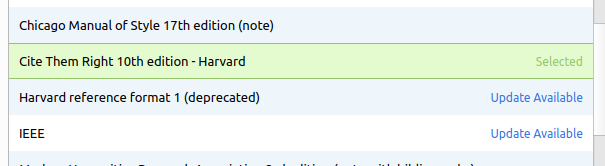
\includegraphics[width=80mm]{pics/cite_them_right.png}%
	\end{itemize}
    \item easy access to PDF to send via emails, if impossible to share via server (Show containing folder, left-click on the attached file in the right-hand bottom corner)
    \item search and merge duplicates (un-checked fields have conflicting data)
\end{enumerate}

\section{Advanced setups and limitations}

\begin{itemize}
	\item watched folder (e.g. Downloads/2mendeley) for files (inc. docx) from non-generic sources
		\begin{itemize}
			\item Tools -> Options -> Watched Folder
		\end{itemize}
	\item BibTex Syncing: export a .bib for each folder
		\begin{itemize}
			\item Tools -> Options -> BibTex
		\end{itemize}
	\item sexy, but an overkill: automatically update (and clean) the bib file in Tex project to integrate changes in a Mendeley folder
	\begin{itemize}
		\item requires editing and running .sh with fswatch (a file change monitor) and editing .py; see \HREF{./manage\_bib/}{manage\_bib} folder for instructions
	\end{itemize}
	
\end{itemize}

\tcbset{colback=yellow!5!white,colframe=yellow!50!black!40}
\begin{tcolorbox}[width=\textwidth, nobeforeafter,valign=center, fonttitle=\Large\bfseries,title=My current issues with Mendeley]
	\begin{enumerate}
		\item no Linux Distribution for the latest September 2020 Mendeley Reference Manager v2.67.0
		\item throwback to Mendeley Desktop after each `insert citation' in LO Writer
		\item noisy/unadjustable bib exports (Tools -> Options -> Document details)
		\item protected input in titles (do you need to stick to the original casing of the publication or do you want consistency in your References?)
		\item bad month format July -> jul
		\item impossible to uncheck some fields that are output by default for Document types in (I don't want to output Abstract, keywords and Mendeley group, file path)
	\end{enumerate}
\end{tcolorbox}

\section{Library use and maintenance}

Useful tips: 

\begin{itemize}
	\item decide on, and set up, the style of your citation keys e.g. [AuthorYear]
	\item download the published version (or replace relevant preprints as they get published) (see \href{https://scholar.google.com/scholar?hl=en\&as\_sdt=0\%2C5\&q=Controlling+Text+Complexity+in+Neural+Machine+Translation\&btnG=}{GoogleScholar options});
	\item update the database;
	\item merge duplicate recordings;
	\item set up Tools -> Options -> Document Details for each type of source
	\item fill in details in full;
	\item clean up `Recently added' and `Unsorted' regularly 
\end{itemize}


\section*{Task 7. Start your own library and/or demonstrate the following}
\label{task}
\addcontentsline{toc}{section}{Task 7. Start your own library}

\begin{tcolorbox}[width=\textwidth, colback={yellow!40!white}, title={}, colbacktitle=yellow!60!white, coltitle=black]
	\begin{itemize}
		\item share a Mendeley folder with mkunilovskaya@gmail.com if you are using Mendeley;
		\item send me an editable document (.docx, .odt) with a screenshot of your library and a sample text with automatically imported in-text citations and plugin-generated References;  
		\item send me a bib exported from one of the folders in your library.
	\end{itemize}
	
\end{tcolorbox}%

\end{document}